\documentclass[tikz,border=4pt]{standalone}
\usepackage{tikz}
\usepackage{pgfplots}
\usepackage{amsmath}
\pgfplotsset{compat=1.18}

\begin{document}
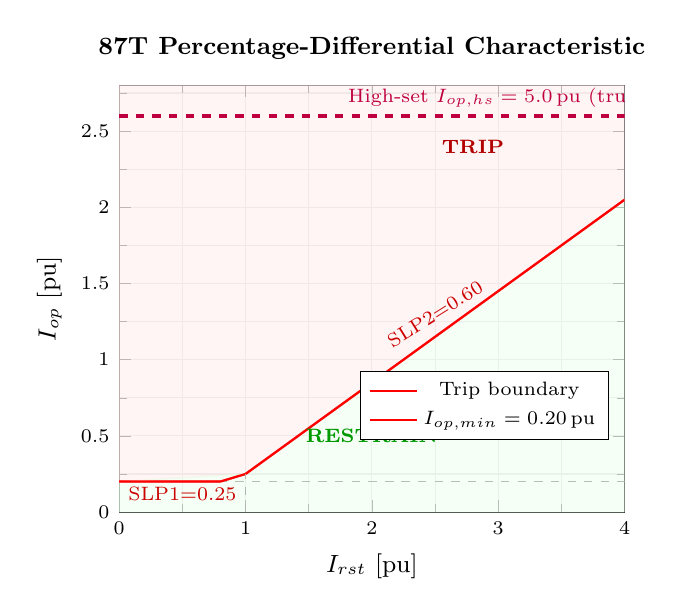
\begin{tikzpicture}
\begin{axis}[
  width=8cm, height=7cm,
  xlabel={$I_{rst}$ [pu]},
  ylabel={$I_{op}$ [pu]},
  xmin=0, xmax=4.0,
  ymin=0, ymax=2.8,
  grid=both,
  grid style={gray!20},
  minor tick num=1,
  tick label style={font=\scriptsize},
  label style={font=\small},
  legend style={font=\scriptsize,at={(0.97,0.25)},anchor=east},
  title style={font=\small\bfseries},
  title={87T Percentage-Differential Characteristic},
]

%% --- Trip boundary (SLP1=0.25 up to I_rst_k=1.0, SLP2=0.60 above) ----------
\addplot[red,thick,domain=0:1.0,samples=50]  {max(0.20, 0.25*x)};
\addplot[red,thick,domain=1.0:4.0,samples=50]
      {max(0.20, 0.25*1.0 + 0.60*(x-1.0))};
\addlegendentry{Trip boundary};

%% --- I_op_min ---
\addplot[gray,dashed,thin,domain=0:4.0] {0.20};
\addlegendentry{$I_{op,min}=0.20$\,pu};

%% --- Operating regions (shaded) --
%% Trip region (above boundary) — light red
\addplot[red!10,fill=red!8,opacity=0.5]
  coordinates {(0,0.20)(1.0,0.25)(4.0,2.05)(4.0,2.8)(0,2.8)(0,0.20)};

%% Restrain region (below boundary) — light green
\addplot[green!10,fill=green!8,opacity=0.5]
  coordinates {(0,0)(4.0,0)(4.0,2.05)(1.0,0.25)(0,0.20)(0,0)};

%% Re-draw boundary on top
\addplot[red,thick,domain=0:1.0,samples=50]  {max(0.20, 0.25*x)};
\addplot[red,thick,domain=1.0:4.0,samples=50]
      {max(0.20, 0.25*1.0 + 0.60*(x-1.0))};

%% --- Slope labels ---
\node[font=\scriptsize,red!80!black] at (axis cs:0.5,0.12) {SLP1=0.25};
\node[font=\scriptsize,red!80!black,rotate=32] at (axis cs:2.5,1.3) {SLP2=0.60};

%% Region labels
\node[font=\scriptsize\bfseries,green!60!black] at (axis cs:2.0,0.5) {RESTRAIN};
\node[font=\scriptsize\bfseries,red!70!black]   at (axis cs:2.8,2.4) {TRIP};

%% Breakpoint
\draw[dashed,gray!60] (axis cs:1.0,0) -- (axis cs:1.0,0.25);
\node[font=\tiny,gray!80] at (axis cs:1.0,-0.12) {$I_{rst,k}=1.0$};

%% --- Unrestrained high-set ---
\draw[purple,ultra thick,dashed]
      (axis cs:0,2.6) -- (axis cs:4.0,2.6);
\node[font=\scriptsize,purple] at (axis cs:3.2,2.72)
      {High-set $I_{op,hs}=5.0$\,pu (truncated)};

\end{axis}
\end{tikzpicture}
\end{document}
